\documentclass[10pt,aspectratio=43,mathserif]{beamer}
\usepackage{nju}			 %导入 nju 模板宏包
%\usepackage[UTF8]{ctex}      %导入 ctex 宏包,添加中文支持
\usepackage{xeCJK}
\usepackage{amsmath,amsfonts,amssymb,bm}   %导入数学公式所需宏包
\usepackage{color}			 %字体颜色支持
\usepackage{graphicx,hyperref,url}
\usepackage{listings}
\usepackage{booktabs}
\usepackage{multirow}
\usepackage{float}

\beamertemplateballitem		%设置 Beamer 主题
\catcode`\。=\active        %或者=13
\newcommand{。}{.}         %将正文中的“。”号转换为“.”。

%\AtBeginSection[]
%{
%  \begin{frame}
%    \frametitle{Contents}
%    \tableofcontents[currentsection]
%  \end{frame}
%}



\title{A Brief Population Analysis on Polarized Water}	        %首页信息设置

\author[]{            %个人信息设置
    Shirong Wang\\[0.3cm]
    %15XXXXXXXX\\[0.3cm]
    Kuang Yaming Honors School}

\date{\today}



\begin{document}

\begin{frame}
\titlepage
\end{frame}

\begin{frame}
\frametitle{Contents}
\tableofcontents
\end{frame}


\section{Non-polarized Water}
\begin{frame}
\frametitle{}
\begin{figure}[H]
	\includegraphics[width=0.4\linewidth]{../CMS/w1.png}
\end{figure}
\begin{table}[H]
	\begin{tabular}{cccc}
		\hline
		Atom charges & Mulliken & NPA & ESP(MK) \\ \hline
		O &-0.642 & -1.011 & -0.877  \\
		H &0.295 & 0.486 & 0.449   \\
		H &0.274 & 0.483 & 0.379   \\
		\hline
		dipole & & & \\
		\hline
	\end{tabular}
	\caption{Atomic charges on each atom of non-polarized water}
\end{table}
All results are calculated under M06-2X/def2-QZVP
\end{frame}
\section{Polarized Water}

\begin{frame}
\frametitle{Configuration I}
\begin{figure}[H]
	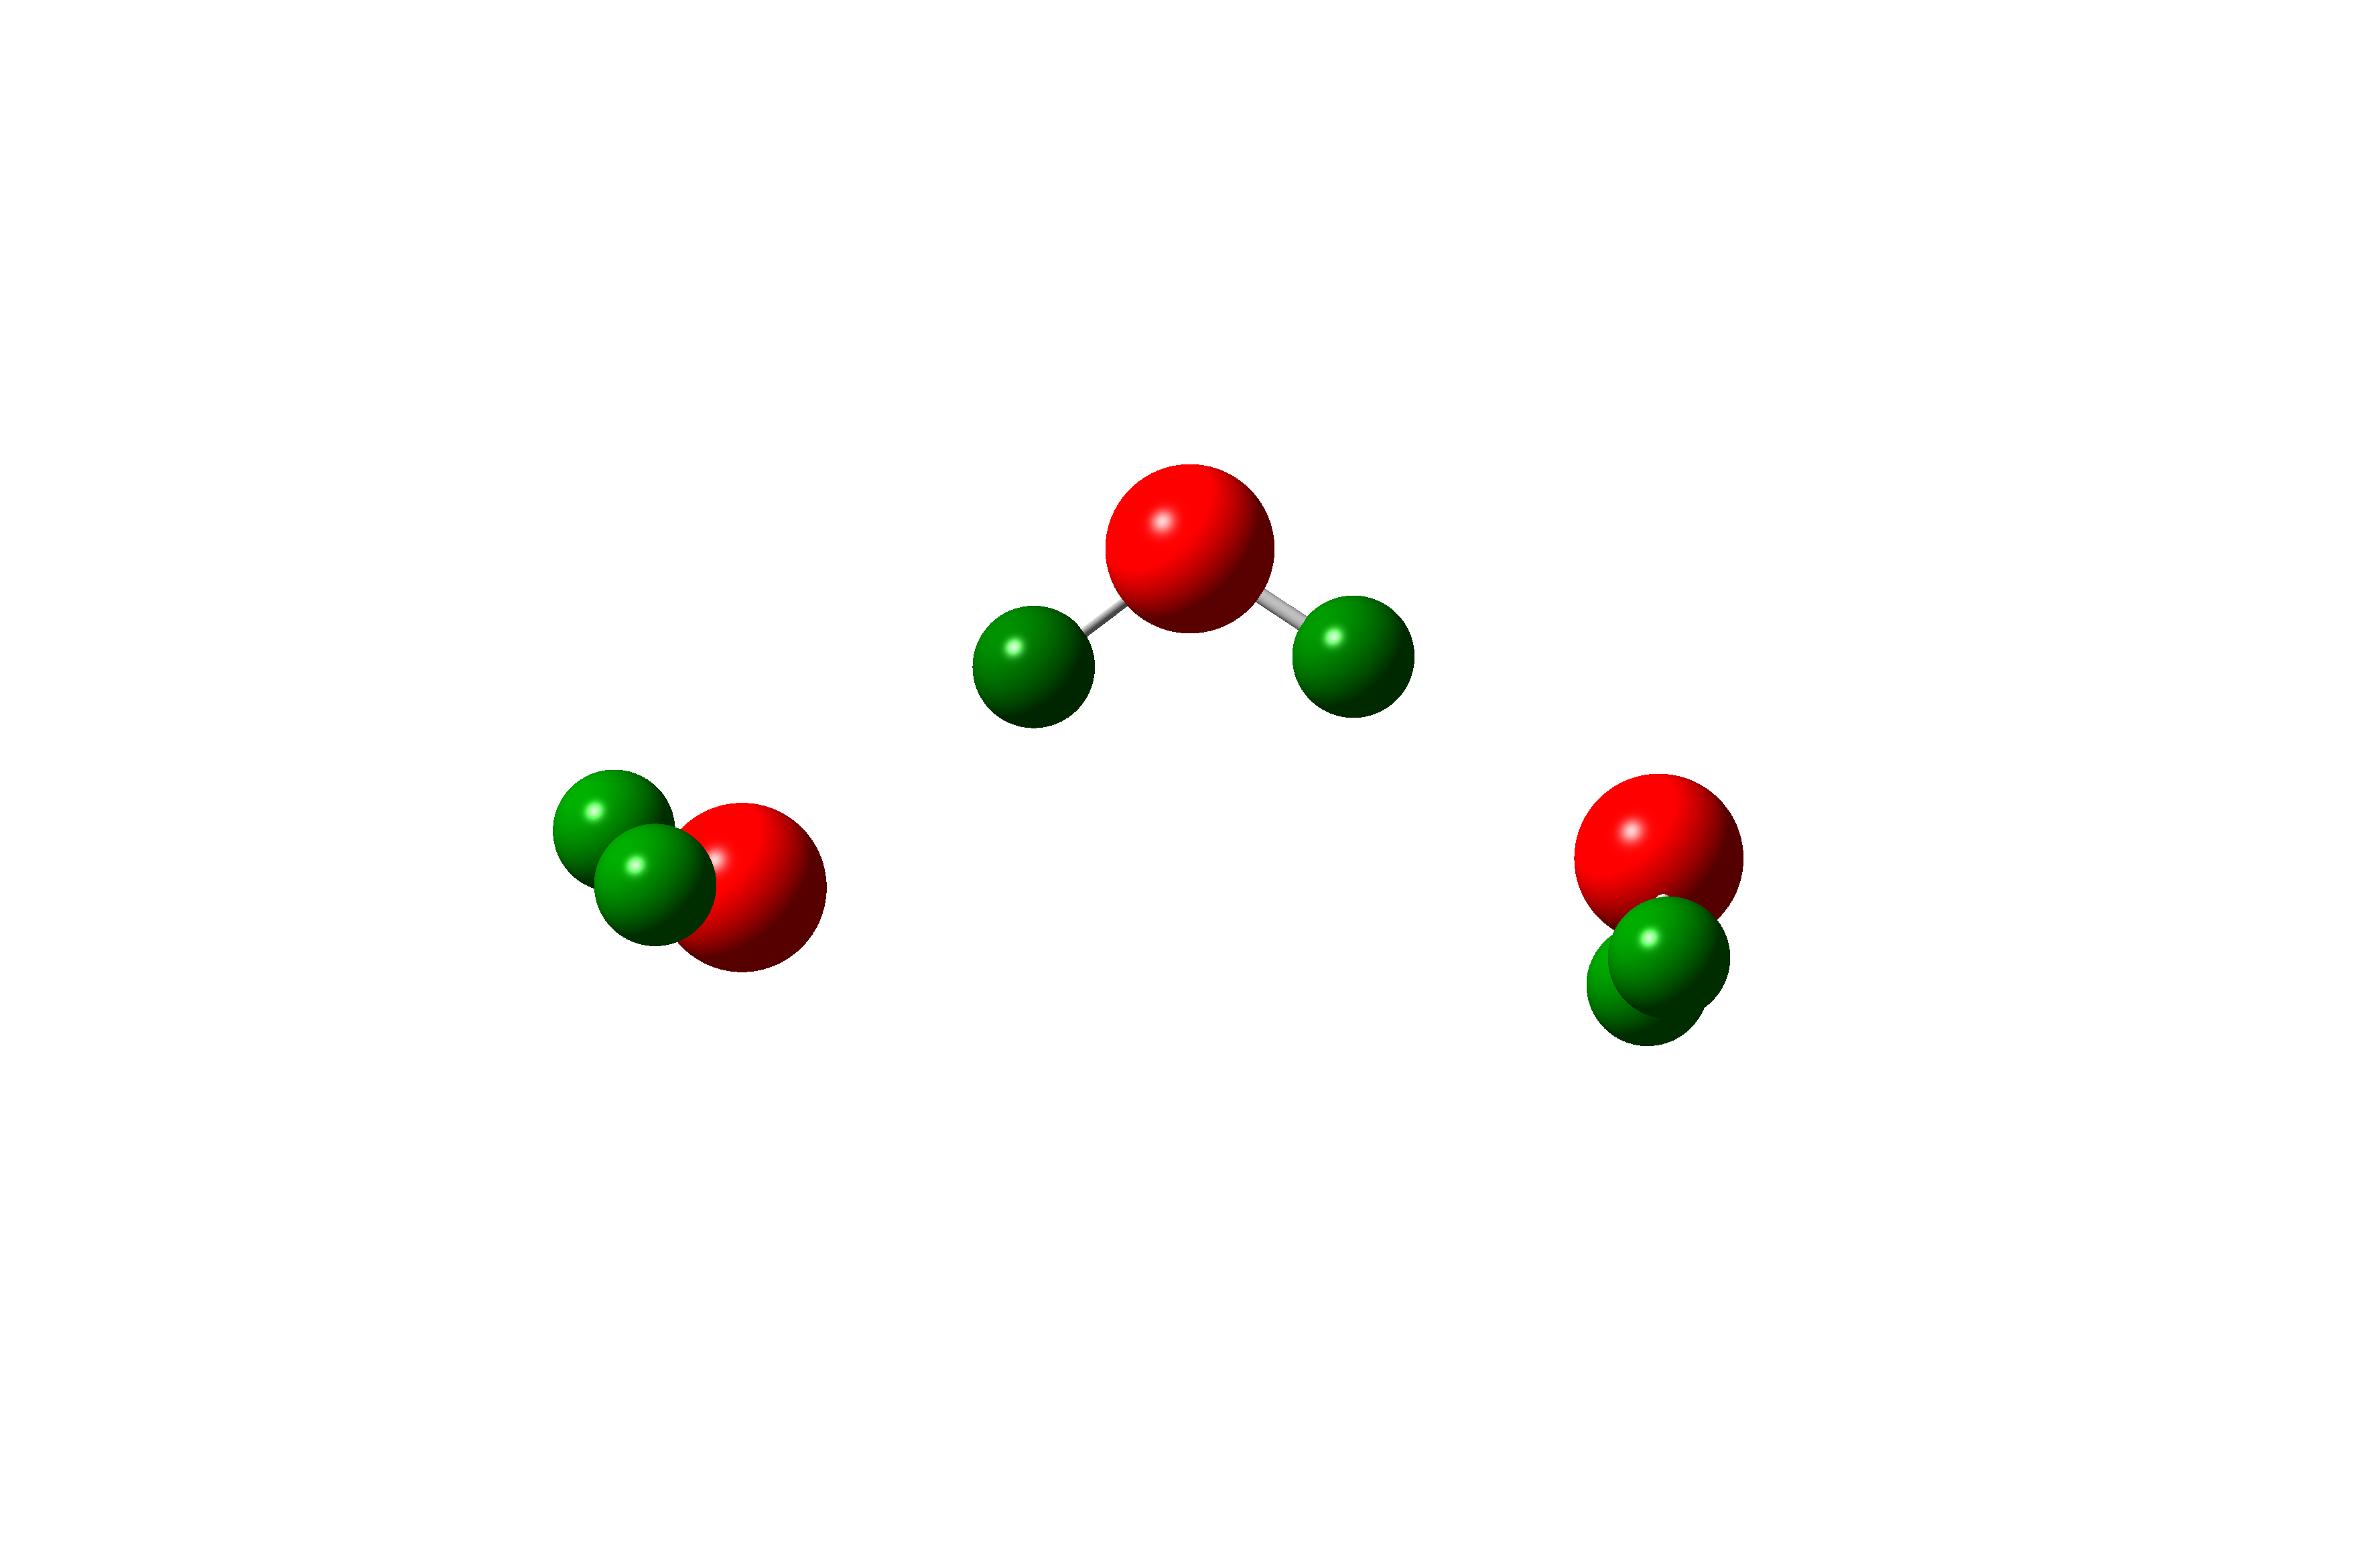
\includegraphics[width=0.4\linewidth]{../CMS/w3bwhite.png}
\end{figure}
\begin{table}[H]
	\begin{tabular}{cccc}
		\hline
		Atom charges & Mulliken & NPA & ESP(MK) \\ \hline
		O &-0.642 & -1.011 & -0.877  \\
		H &0.295 & 0.486 & 0.449   \\
		H &0.274 & 0.483 & 0.379   \\
		\hline
		dipole & & & \\
		\hline
	\end{tabular}
	\caption{Atomic charges on each atom of polarized water}
\end{table}
\end{frame}

\begin{frame}
\frametitle{Configuration II}
\begin{figure}[H]
	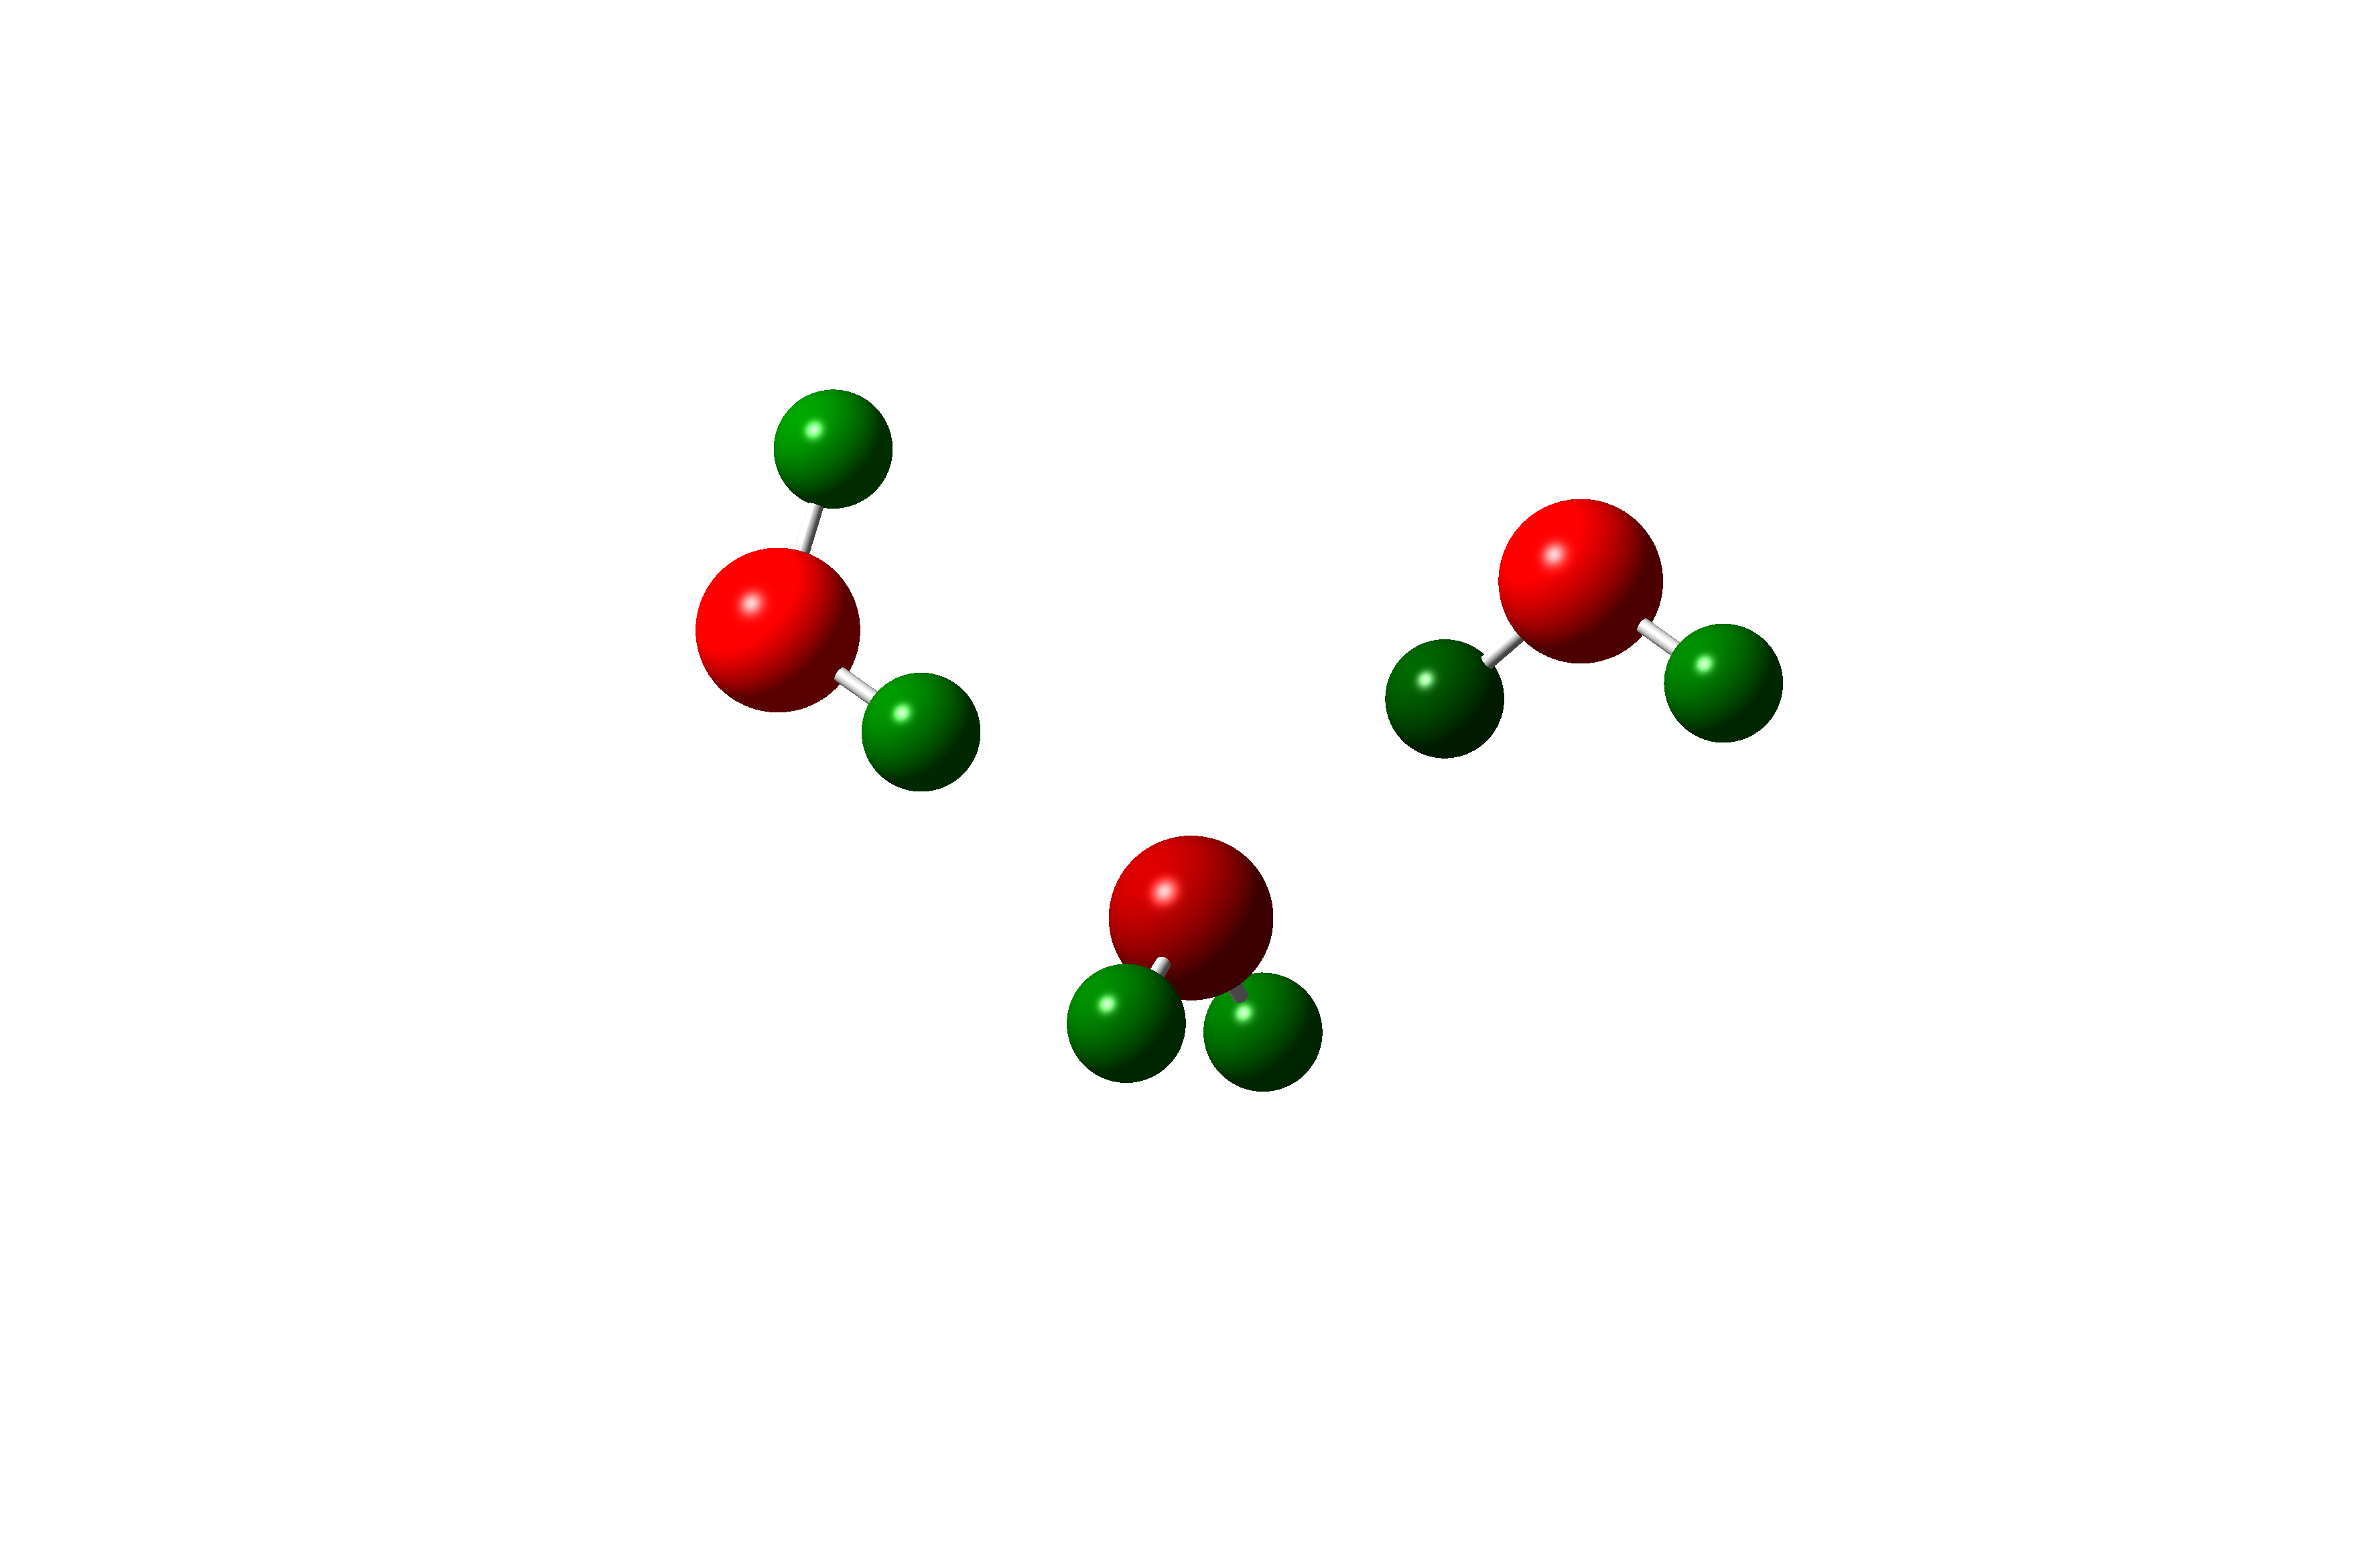
\includegraphics[width=0.4\linewidth]{../CMS/w3cw.png}
\end{figure}
\begin{table}[H]
	\begin{tabular}{cccc}
		\hline
		Atom charges & Mulliken & NPA & ESP(MK) \\ \hline
		O &-0.655 & -0.950 & -0.550  \\
		H &0.353 & 0.496 & 0.358   \\
		H &0.352 & 0.495 & 0.341   \\
		\hline
		dipole & & & \\
		\hline
	\end{tabular}
	\caption{Atomic charges on each atom of polarized water}
\end{table}
\end{frame}


\section{第二章标题}




\begin{frame}[c, plain]
  \begin{center}
    \Huge{\texttt{\textbf{Thank you!}}}\\[0.5cm]
    Q\&A
  \end{center}
\end{frame}


\end{document}
